\documentclass[10pt, aspectratio=169]{beamer}

% --- Typography & Colors ---
\usepackage[sfdefault]{FiraSans} 
\usepackage[T1]{fontenc}
\usepackage[utf8]{inputenc}
\usepackage{booktabs} 
\usepackage{tikz}

\definecolor{AcademicNavy}{RGB}{0, 51, 102}
\setbeamercolor{titlelike}{fg=AcademicNavy}
\setbeamercolor{structure}{fg=AcademicNavy}

% --- Custom Title Page Design ---
\setbeamertemplate{title page}{
    \vspace*{0.5cm}
    % 1. TOP Logo Header
    \begin{columns}[c, totalwidth=\textwidth]
        \column{0.20\textwidth}
            \raggedright
\includegraphics[height=1.0cm]{LOGO_CNRS_BLEU.png}
        \column{0.60\textwidth}
            \centering
\includegraphics[height=1.0cm]{logo_lspm.png}
        \column{0.20\textwidth}
            \raggedleft
\includegraphics[height=1.0cm]{USPN.png}
    \end{columns}

    \vspace{0.8cm}

    % 2. Title and Subtitle Block
    \begin{centering}
        {\usebeamerfont{title} \usebeamercolor[fg]{title} \huge \textbf{\inserttitle} \par}
        \vspace{0.4cm}
        {\usebeamerfont{subtitle} \usebeamercolor[fg]{subtitle} \small \textit{\insertsubtitle} \par}
        
        \vspace{0.5cm}
        
        {\usebeamerfont{author} \large \textbf{\insertauthor} \par}
        \vspace{0.15cm}
        {\usebeamerfont{institute} \tiny \insertinstitute \\[0.1cm] \scriptsize \insertdate \par}
    \end{centering}

    \vspace{0.4cm}

    % 3. Jury Panel (Aligned Footer)
    \begin{columns}[T, onlytextwidth]
        \begin{column}{0.48\textwidth}
            {\tiny \color{AcademicNavy}\textbf{Rapporteurs}\\[0.1cm]
            \begin{tabular}{@{}p{3.0cm} l@{}}
                Mme Maurine MONTAGNAT & \textit{DR CNRS, IGE} \\
                M. Muhittin MUNGAN & \textit{Professeur, Univ. of Cologne} \\
                M. Aurélien VATTRÉ & \textit{MR Onera, Univ. Paris-Saclay} \\
            \end{tabular}}
        \end{column}
        \hfill
        \begin{column}{0.48\textwidth}
            {\tiny \color{AcademicNavy}\textbf{Examinateurs}\\[0.1cm]
            \begin{tabular}{@{}p{3.0cm} l@{}}
                Mme Véronique LAZARUS & \textit{Professeure, ENSTA Paris} \\
                M. Nicolas AUFFRAY & \textit{Professeur, Sorbonne Université} \\
                M. Denis GRATIAS & \textit{DR émérite CNRS, IRCP} \\
                M. Damien FAURIE & \textit{Professeur, USPN} \\
                M. Ioan R. IOANESCU & \textit{Professeur, USPN} \\
            \end{tabular}}
        \end{column}
    \end{columns}

    \vspace{0.5cm}
}


% --- Metadata ---
\title{Mechanics of displacive instabilities in solids}
\subtitle{Habilitation à Diriger des Recherches (HDR)}
\author{O\u{g}uz Umut Salman}
\institute{Laboratoire des Sciences des Procédés et des Matériaux (LSPM) \\ CNRS UPR 3407 | Université Sorbonne Paris Nord}
\date{31 Mars 2026}

\begin{document}

% Slide 1
\begin{frame}[plain]
    \titlepage
\end{frame}

% Slide 2
\section{Introduction}
\begin{frame}{Scientific Context: Nonlinearity \& Instability}
    \begin{columns}[c]
        \column{0.6\textwidth}
        \textbf{The Challenge:} 
        Understanding material behavior beyond the elastic limit where microscale rearrangements drive macroscopic nonlinearity.
        
        \vspace{0.3cm}
        \textbf{Key Phenomena:}
        \begin{itemize}
            \item \textbf{Phase Transitions:} Martensitic transformations.
            \item \textbf{Plasticity:} Dislocation-mediated flow and avalanches.
            \item \textbf{Fracture:} Brittle-to-ductile transitions and damage.
        \end{itemize}
        
        \column{0.4\textwidth}
        
        \begin{block}{Unifying Perspective}
            Treating these diverse phenomena as \textit{displacive instabilities} driven by the competition between elastic energy and lattice symmetry.
        \end{block}
    \end{columns}
\end{frame}

% Slide 3
\begin{frame}{Non-linear phenomena}
    \begin{columns}[T, onlytextwidth]
        % Left Column: Crystals
        \begin{column}{0.48\textwidth}
            \begin{block}{Crystals (PDFs)}
                \centering
                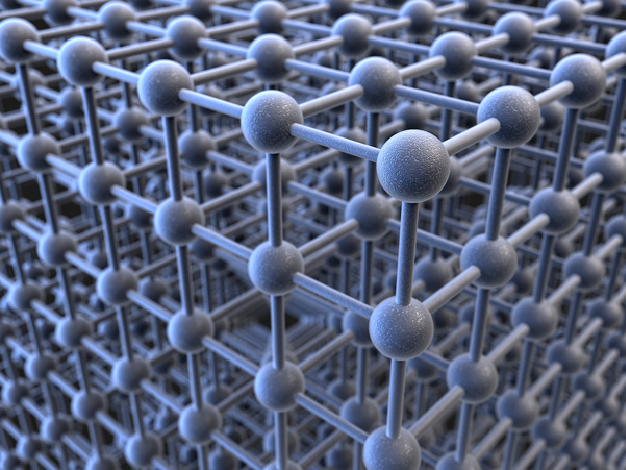
\includegraphics[width=0.45\textwidth]{Figures/crystal.pdf}
                \hspace{0.1cm}
                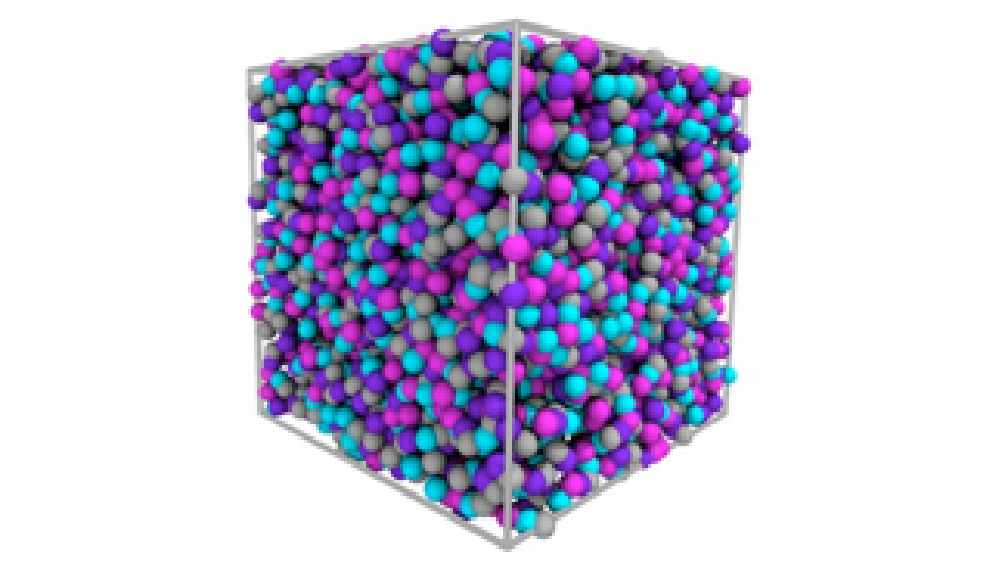
\includegraphics[width=0.45\textwidth]{Figures/amorphous.pdf}
                \\[0.2cm]
                {\tiny Solid-to-solid transitions in lattice structures.}
            \end{block}
        \end{column}

        \hfill

        % Right Column: Meta-materials (Architected)
        \begin{column}{0.48\textwidth}
            \begin{block}{Meta-materials (PNGs)}
                \centering
                
\includegraphics[width=0.45\textwidth]{Figures/Page3_Fig1.png}
                \hspace{0.1cm}
                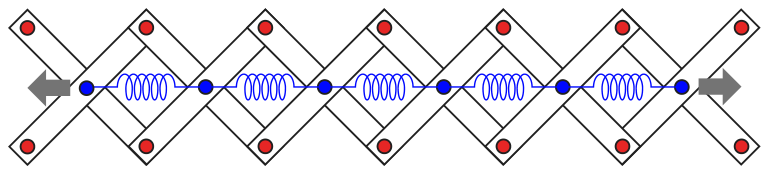
\includegraphics[width=0.45\textwidth]{Figures/Page5_Fig1.png}
                \\[0.2cm]
                {\tiny Structural rearrangements in architected materials.}
            \end{block}
        \end{column}
    \end{columns}
\end{frame}

\end{document}